\section{introduction}
\label{sec:component_diagrams-introduction}

The CODA tooling consists of a plug-in for the Rodin toolset. The plug-in provides a Component Diagram modelling tool, which enables component models to be added as an extension to an Event-B machine. A translator is provided to generate Event-B elements in the machine that implements the behaviour expressed in the Component Diagram. Hence the Component model contributes additional variables, invariants, guards and actions to the existing Event-B model and its events. The component model also generates a timer event and associated synchronisation infrastructure to the model. The component model makes use of and integrates with the existing Event-B State-machines  modelling tool, which is similarly designed to contribute behaviour to existing events.

\subsection{Basis}
As Rodin is an Eclipse based tool, so is CODA. The CODA tooling is based on the Event-B EMF framework, Event-B EMF Extensions and Generic Diagrams plug-ins .

\subsection{The CODA Meta-model}
Key:
\begin{itemize}
\item  RED - Concrete Meta-class,
\item  YELLOW - Abstract Meta-class,
\item  GREEN - Referenced meta-class from another domain meta-model
\end{itemize}


\begin{figure}[!htbp]
  \centering
  \ifplastex
  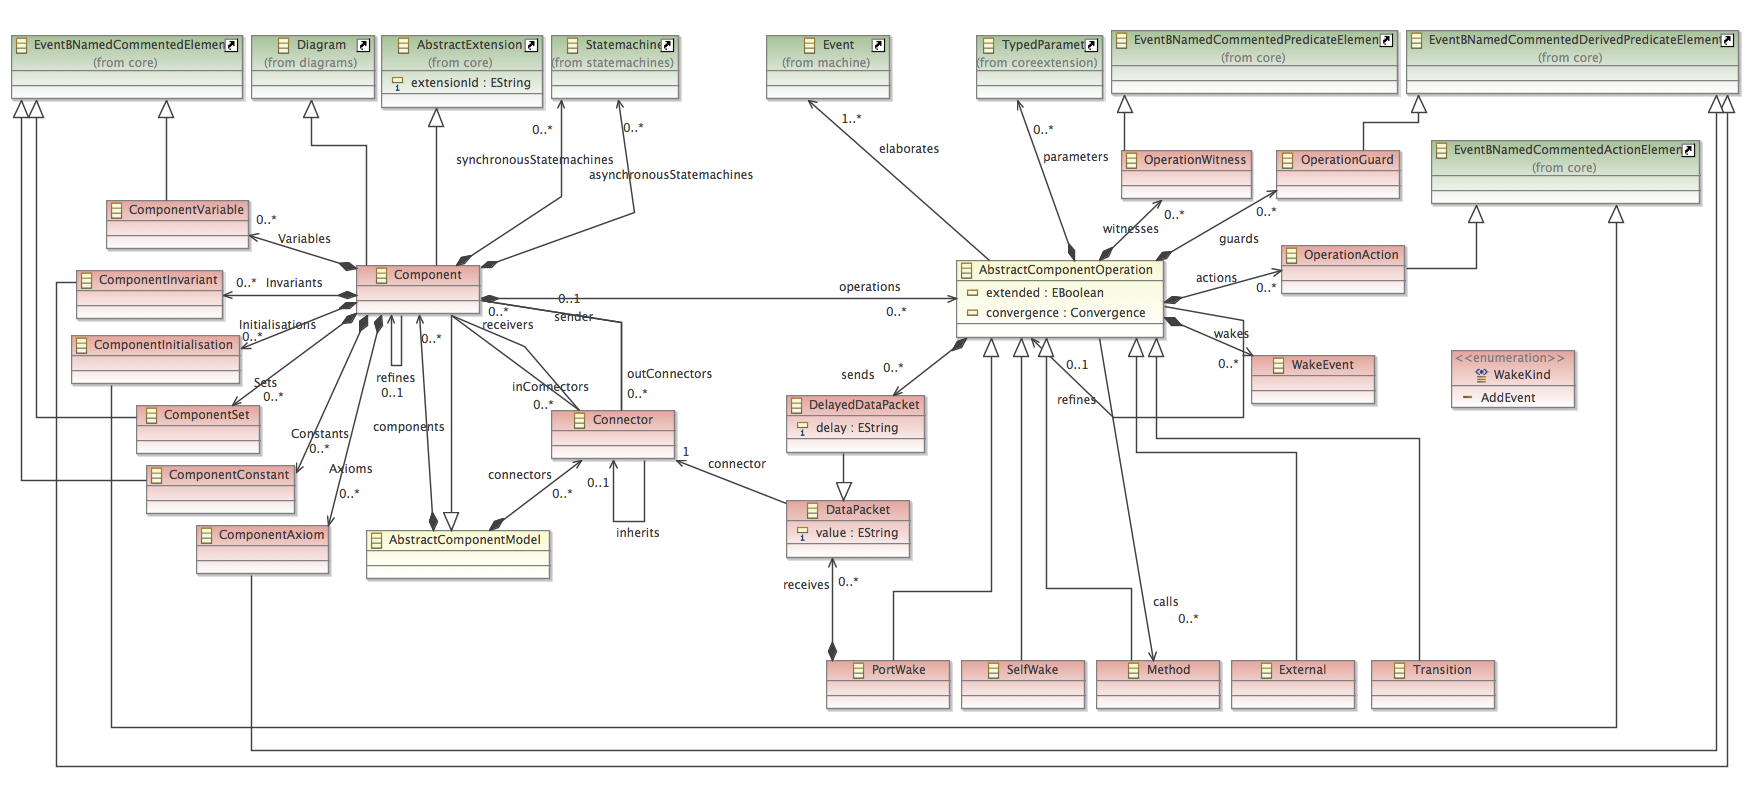
\includegraphics[width=1024]{figures/image1.png}
  \else
  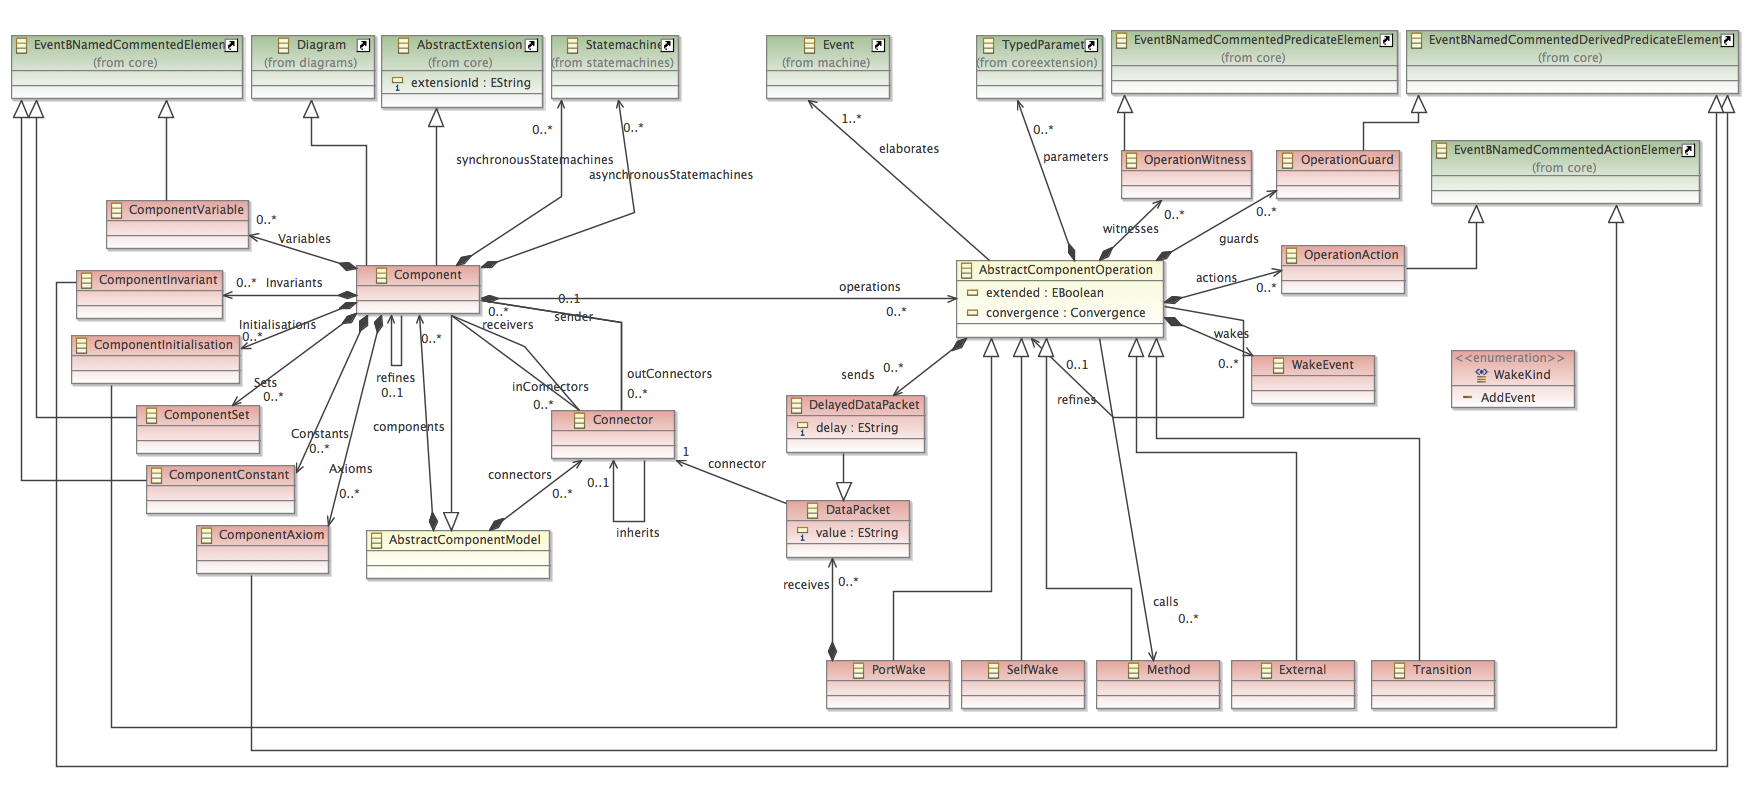
\includegraphics[width=1.0\textwidth]{figures/image1.png}
  \fi
  \caption{The CODA Meta-model}
  \label{fig:TheCodaMetamodel}
\end{figure}



The CODA Meta-model (Figure \ref{fig:TheCodaMetamodel}) defines an abstract syntax for the modelling language.
The boxes (called meta-classes) represent classes of elements that a particular CODA model might have.
In the diagram, the meta-classes are colour coded as follows.
Green indicates a referenced meta-class from another, more general, meta-model (i.e. not part of CODA), 
yellow indicates an abstract meta-class which can not be instantiated directly, but may be instantiated through one of its concrete specialised meta-classes and 
red indicates a concrete CODA meta-class that can be directly instantiated. 
These meta-classes are linked in three different kinds of ways:

\begin{itemize}
\item Generalisation indicates that instances of the source class are also instances of the target class. The targets properties are inherited by any meta-classes that specialise it.  For example, the meta-classes, \emph{PortWake}, \emph{SelfWake}, \emph{Method} etc. all specialise \emph{AbstractComponentOperation} so that operation properties such as \emph{sends} and \emph{wakes} do not have to be defined repeatedly. 
\item Containment indicates that instances of the source meta-class own instances of the target meta-class in a parent-child relationship. For example, any \emph{Component} may own a collection of\emph{AbstractComponentOperation}, which is referred to collectively as its \emph{operations}. 
\item Reference indicates that instances of the source meta-class may reference instances of the target meta-class. For example, any \emph{AbstractComponentOperation} may reference several\emph{Methods} via its \emph{calls} property although it does not contain them as children. 
\end{itemize}


%%% Local Variables:
%%% mode: latex
%%% TeX-master: "component_diagrams-user_manual"
%%% End:
